\begin{figure}[h]
\centering
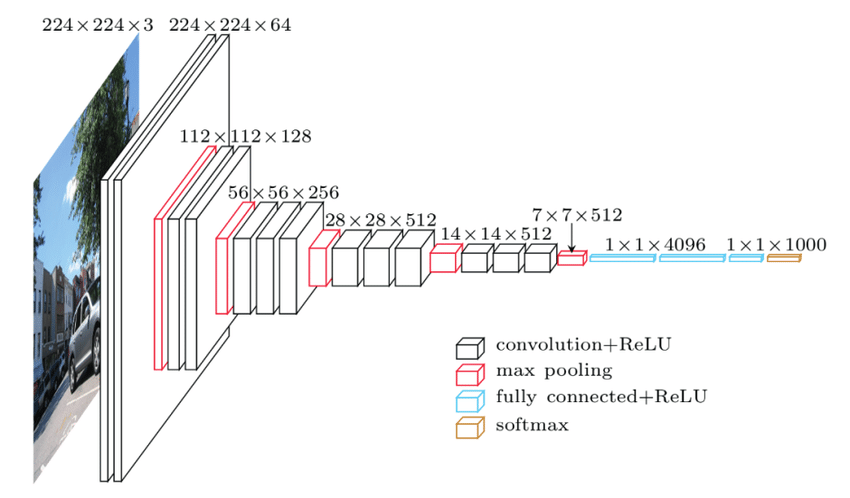
\includegraphics[width=.8\textwidth]{images/Chapter2/VGGNet-architecture-19.png}
\caption{Architecture of a VGG16 network. The input image is processed by 13 convolutions with a kernel size of 3x3. After the first two convolutions, a max pooling halves the resolution but doubles the amount of filters \citep{Bezdan_2019}.} 
\label{fig:vgg16}
\end{figure}

The 2015 introduced architecture for deep learning by the Visual Geometry Group of Oxford University (VGG) was one of the first networks that was able to get higher accuracies than shallower networks. \citet{Simonyan_2015} found out that two convolutions with a 3x3 kernel have the same field of view as one 5x5 kernel and three 3x3 kernels as one 7x7 respectively. The big improvement however was, that the number of parameters with three 3x3 kernels is considerably ($81\%$) lower than the number of parameters of one 7x7 kernel. This allows efficiency despite the network's depth. It is important to mention that this might come with possible disadvantages. Because of the change in kernel size, we might end up restricting our solution area. This will be neglected however, because it is not possible to test the two kernel sizes against each other. I will assume that the accuracy does not suffer from this effect.  Because VGG was developed for the ILSVRC which consists of 1000 classes, the convolution output is fed into two fully connected dense networks with 4096 channels each and a third and final dense network with 1000 outputs and a softmax activation function \eqref{softmax}. Softmax is another very common activation function, giving the probability of each output neuron and thus the probability for each of the 1000 image classes.

\begin{equation}
    f(\pmb{z})_i = \frac{e^{z_i}}{\sum_{j=1}^{K} e^{z_j}}, \; \;  \text{for} \; i=1 \; \; \text{and} \; \; \pmb{z} = (z_1,\ldots,z_K)
\label{softmax}
\end{equation}

The authors provide two different version of their network. VGG16 (\autoref{fig:vgg16}) consists of 16 total layers with 134 million parameters and VGG19 consists of 19 layers with 144 million parameters. For VGG19, the first two convolution layers are the same as for VGG16, but the next three have one additional convolution. The dense networks remain unchanged. The slightly deeper VGG19 was able to perform a little bit better than the shallower VGG16, scoring around $0.1\%$ less top-5 validation error thorughout multiple tests.